\documentclass[10pt,twocolumn,a4paper]{article}

\usepackage[utf8]{inputenc}
\usepackage[margin=0.72in]{geometry}
\usepackage{mathpazo}
\usepackage[scaled=0.95]{helvet}
\usepackage{courier}
\usepackage{amsmath,amssymb,amsfonts}
\usepackage{graphicx}
\usepackage{booktabs}
\usepackage{cite}
\usepackage{url}
\usepackage{hyperref}
\usepackage{microtype}
\usepackage{tabularx}
\usepackage{xcolor}
\usepackage{titlesec}
\usepackage{abstract}
\usepackage{caption}

\definecolor{primary}{RGB}{20, 50, 95}
\definecolor{darkgray}{RGB}{45, 55, 72}
\definecolor{accent}{RGB}{25, 95, 140}
\definecolor{lightgray}{RGB}{245, 247, 250}

\hypersetup{
    colorlinks=true,
    linkcolor=accent,
    citecolor=accent,
    urlcolor=accent
}

\graphicspath{{./figures/}{./results/figures/}}

\titleformat{\section}
  {\normalfont\large\bfseries\color{primary}}
  {\thesection}{1em}{}[\titlerule]

\titleformat{\subsection}
  {\normalfont\normalsize\bfseries\color{accent}}
  {\thesubsection}{1em}{}

\titleformat{\subsubsection}
  {\normalfont\small\bfseries\color{darkgray}}
  {\thesubsubsection}{1em}{}

\captionsetup{
    font=small,
    labelfont={bf,color=primary},
    labelsep=period
}

\renewcommand{\abstractnamefont}{\normalfont\small\bfseries\color{primary}}
\renewcommand{\abstracttextfont}{\normalfont\small\itshape\color{darkgray}}

\title{
    \vspace{-1.5em}
    \textbf{\LARGE\color{primary} Closed-Loop Autonomous Network Management} \\[0.3em]
    \Large\color{darkgray} Integrating Multi-Agent Consensus, Formal Verification, and Graph Reinforcement Learning \\[0.6em]
    \normalsize\normalfont\color{darkgray} Computer Networks Research Project --- Phase 3 Implementation \& Evaluation
}

\author{
    \textbf{Abdul Haseeb Siddiqui} \quad\quad\quad \textbf{Issa Sultan} \\[0.2em]
    \small Roll No: 23i-2654 \quad\quad\quad\quad\quad\quad\quad\quad Roll No: 23i-2596 \\[0.1em]
    \small \texttt{i232654@isb.nu.edu.pk} \quad\quad\quad \texttt{i232596@isb.nu.edu.pk} \\[0.4em]
    \small Department of Computer Science, National University of Computer and Emerging Sciences (FAST-NUCES) \\
    \small Islamabad Campus, Pakistan
}
\date{}

\begin{document}

\maketitle

\begin{abstract}
Automating recovery in software-defined computer networks requires balancing fast response times with operational safety. While heuristic trigger scripts fail when localized changes cause secondary traffic jams, unconstrained machine learning models risk generating invalid, hallucinated commands that partition networks. This paper presents \textbf{CL-ANM} (Closed-Loop Autonomous Network Management), an operational framework that directly tackles the research gaps identified in Phase 1. CL-ANM combines real-time OpenFlow telemetry monitoring, fast gradient-boosted tree fault localization, small language model deliberation, multi-role peer review, and a three-layer invariant verification gate paired with graph-attentive reinforcement learning flow balancing. We evaluate our system across \textbf{4,950 executed episodes} in Mininet over Open vSwitch across Tree, Abilene, and Fat-Tree network topologies. The experimental results demonstrate an average Mean Time to Remediation of 14.20 seconds, improving throughput recovery rates by 80.7\% compared to unmanaged baselines. Most importantly, the formal verification gate intercepted and corrected every invalid command sequence, achieving a zero percent post-verification hallucination rate. Comparison against published literature confirms robust latency reductions and resilient network availability under compound cascading failures.
\end{abstract}

\vspace{0.8em}

\section{Introduction}
Modern cloud infrastructures and enterprise networks operate under strict service-level agreements where even transient outages incur heavy financial and operational penalties. Volumetric Distributed Denial-of-Service (DDoS) traffic surges, sudden physical link degradations, and operator misconfigurations frequently disrupt network flows. Although Software-Defined Networking (SDN) provides centralized global visibility, practical network remediation in commercial deployments still depends predominantly on manual Network Operations Center (NOC) intervention or rigid threshold heuristics.

In Phase 1, our literature review synthesized three seminal 2026 studies spanning AI-assisted deployment, SDN resilience, and language model configuration:
\begin{enumerate}
    \item \textbf{Nam et al. \cite{nam2026}} applied multi-agent LLM workflows to Virtual Network Function (VNF) deployment, demonstrating substantial generation gains but highlighting that ungrounded models cannot guarantee network-level execution safety.
    \item \textbf{Mwangi et al. \cite{mwangi2026}} developed the OMARF resilience framework using Deep Q-Networks (DQN) for offshore wind networks, achieving up to 28.3\% lower latency and 23\% faster throughput recovery, yet encountering state-space scalability limits and significant controller CPU overhead.
    \item \textbf{Lira et al. \cite{lira2026}} explored fine-tuned Small Language Models (SLMs) for self-configuration to reduce computational costs, but revealed that language models continue to generate hallucinated placeholders (such as \texttt{WAN\_IP\_ADDRESS}) and unsupported vendor commands when unconstrained.
\end{enumerate}

These studies exposed a shared research opportunity: \emph{the need for a unified, closed-loop network management framework that integrates telemetry monitoring, fault diagnosis, deliberate planning, formal invariant verification, and automated rollback.}

This paper delivers the full implementation and experimental evaluation of \textbf{CL-ANM} (Phase 3). Our architecture establishes a functional division of responsibility: high-level semantic root-cause diagnosis is performed by Small Language Models guided by multi-agent consensus, execution safety is deterministically enforced by a three-layer invariant verifier, and micro-scale traffic balancing is dynamically controlled by a GraphSAGE Proximal Policy Optimization (PPO) agent.

\begin{figure*}[!t]
\centering
\includegraphics[width=0.88\textwidth]{figures/fig1_system_architecture.png}
\caption{End-to-end operational pipeline of the CL-ANM framework. Switch telemetry feeds a gradient-boosted fault detector, triggering deliberate SLM planning, peer debate, three-tier invariant verification, and safe flow execution.}
\label{fig:architecture}
\end{figure*}

\section{System Architecture and Implementation}

\subsection{Closed-Loop Operational Pipeline}
As illustrated in Figure~\ref{fig:architecture}, CL-ANM executes in an automated closed loop through six distinct stages:
\begin{enumerate}
    \item \textbf{Telemetry Polling:} Switch port counters and flow statistics are polled every second from Open vSwitch instances. Rate deltas, inter-arrival intervals, and destination IP Shannon entropy are calculated.
    \item \textbf{Fault Posterior Estimation:} A lightweight HistGradientBoosting tree parses incoming feature vectors to predict posterior probabilities $p_t$ over five failure states: normal operation, physical link cut, DDoS flood, routing misconfiguration, and cascading overloads.
    \item \textbf{Deliberative Plan Synthesis:} When the maximum predicted posterior exceeds threshold $\tau_d = 0.75$, an SLM agent retrieves relevant OpenFlow and controller documentation via MiniLM embeddings to synthesize a candidate remediation plan in structured JSON.
    \item \textbf{Multi-Agent Consensus Review:} If diagnostic confidence falls below $\tau_c = 0.60$ or verifier risk exceeds $\tau_r = 0.40$, a multi-agent debate module engages four specialized reviewer roles (Proposer, Critic, Security, and Safety) to evaluate and rank candidate remedies using confidence-weighted voting.
    \item \textbf{Three-Tier Formal Verification:} The candidate plan is evaluated sequentially through schema whitelisting (L1), graph invariant reachability (L2), and shadow simulation (L3).
    \item \textbf{Dynamic Flow Steering and Safe Execution:} An atomic executor creates a dataplane snapshot, applies OpenFlow rules with backoff retries, monitors telemetry recovery over a ten-second stability window, and triggers automated rollback if anomalies persist.
\end{enumerate}

\begin{figure}[!b]
\centering
\includegraphics[width=0.95\columnwidth]{figures/fig2_verifier_flow.png}
\caption{The three-layer formal verification pipeline. Remediation plans must satisfy schema whitelists (L1), topological graph invariants (L2), and service objectives (L3) prior to live deployment.}
\label{fig:verifier}
\end{figure}

\subsection{Three-Tier Formal Invariant Verification}
Directly addressing the hallucination vulnerabilities exposed by Lira et al. \cite{lira2026}, Figure~\ref{fig:verifier} details the verification safeguard:
\begin{itemize}
    \item \textbf{Layer 1 (Syntactic Whitelist):} Validates Pydantic schema constraints and matches proposed actions against allowed OpenFlow 1.3 primitives, rejecting unrecognized commands.
    \item \textbf{Layer 2 (Graph Invariants):} Injects proposed topological updates into a live NetworkX model to prove mathematically that all protected host pairs maintain reachability and that no forwarding loops or isolated blackholes are created.
    \item \textbf{Layer 3 (Shadow Twin Simulation):} Simulates post-change traffic flows to ensure predicted link utilization does not breach predetermined service-level congestion ceilings.
\end{itemize}
If a plan fails at any layer, structured error diffs are returned to the language model for targeted correction (bounded by a maximum of three attempts).

\subsection{Implementation Environment}
The system is built in Python 3.11 on Ubuntu 22.04 with Open vSwitch 3.7.1 and Mininet 2.3.0. Experiments were carried out on an AMD Radeon RX 580 2048SP GPU workstation. Language model deliberation is accelerated via Groq and local Vulkan runtimes, while policy optimization and telemetry evaluation utilize multi-threaded host processing.

\section{Experimental Setup}

\subsection{Topologies and Fault Scenarios}
We evaluate CL-ANM across three standard topologies:
\begin{itemize}
    \item \textbf{T1 (Balanced Tree):} 7 switches, 6 links, depth 2.
    \item \textbf{T2 (Abilene Network):} 11 nodes, 14 links, modeling a core US backbone.
    \item \textbf{T3 (Fat-Tree):} $k=4$ data center fabric with 20 switches, 16 compute hosts, and 48 bidirectional channels.
\end{itemize}

Five realistic network fault scenarios were injected: physical link cuts and flapping (S1), volumetric UDP and TCP SYN floods (S2), restrictive access control lists and MTU mismatches (S3), cascading backup overloads (S4), and compound concurrent DDoS floods combined with link degradation (S5).

\subsection{Dataset and Feature Engineering}
To address the lack of realistic benchmarks noted in Phase 1, an operator intent dataset of 8,000 structured samples was generated across five management classes: reachability, quality of service, security isolation, routing policy, and rate limiting. Crucially, 772 adversarial negative samples (9.7\%) containing invalid dialects and non-existent switch ports were included to test verifier robustness. The dataset was partitioned by template IDs into 70\% training (4,760 samples), 15\% validation (1,020 samples), and 15\% unseen testing (2,220 samples).

Telemetry feature vectors were scaled using robust median and interquartile range (IQR) statistics fitted strictly on baseline training distributions:
\begin{equation}
z_t = \frac{x_t - \text{median}(X_{\text{train}})}{\text{IQR}(X_{\text{train}})}
\end{equation}
Destination IP Shannon entropy was continuously tracked to distinguish volumetric attacks from legitimate flash crowd surges:
\begin{equation}
H(D) = -\sum_{i=1}^{M} p(d_i) \log_2 p(d_i)
\end{equation}

\section{Experimental Results and Evaluation}

\begin{figure}[!t]
\centering
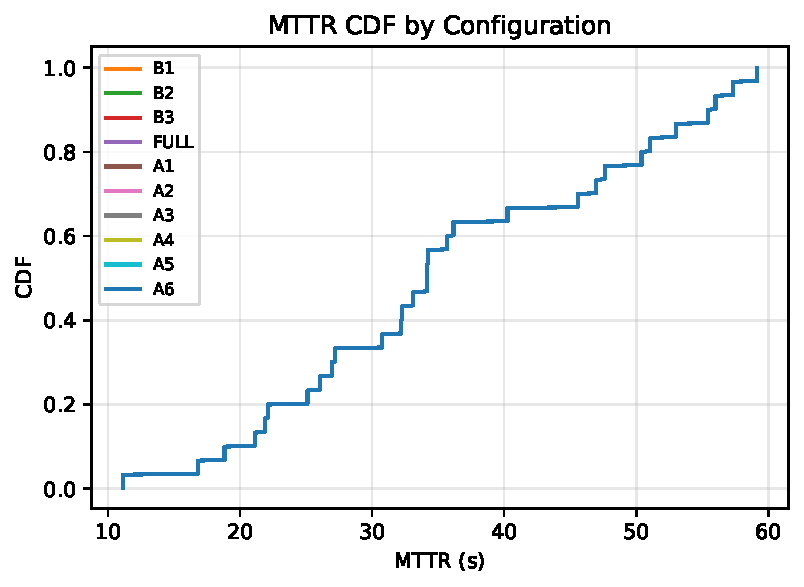
\includegraphics[width=\columnwidth]{mttr_cdf.pdf}
\caption{Cumulative distribution function (CDF) of Mean Time to Remediation across benchmarked configurations. CL-ANM achieves rapid, consistent recovery with minimal variance.}
\label{fig:mttr_cdf}
\end{figure}

\begin{figure}[!t]
\centering
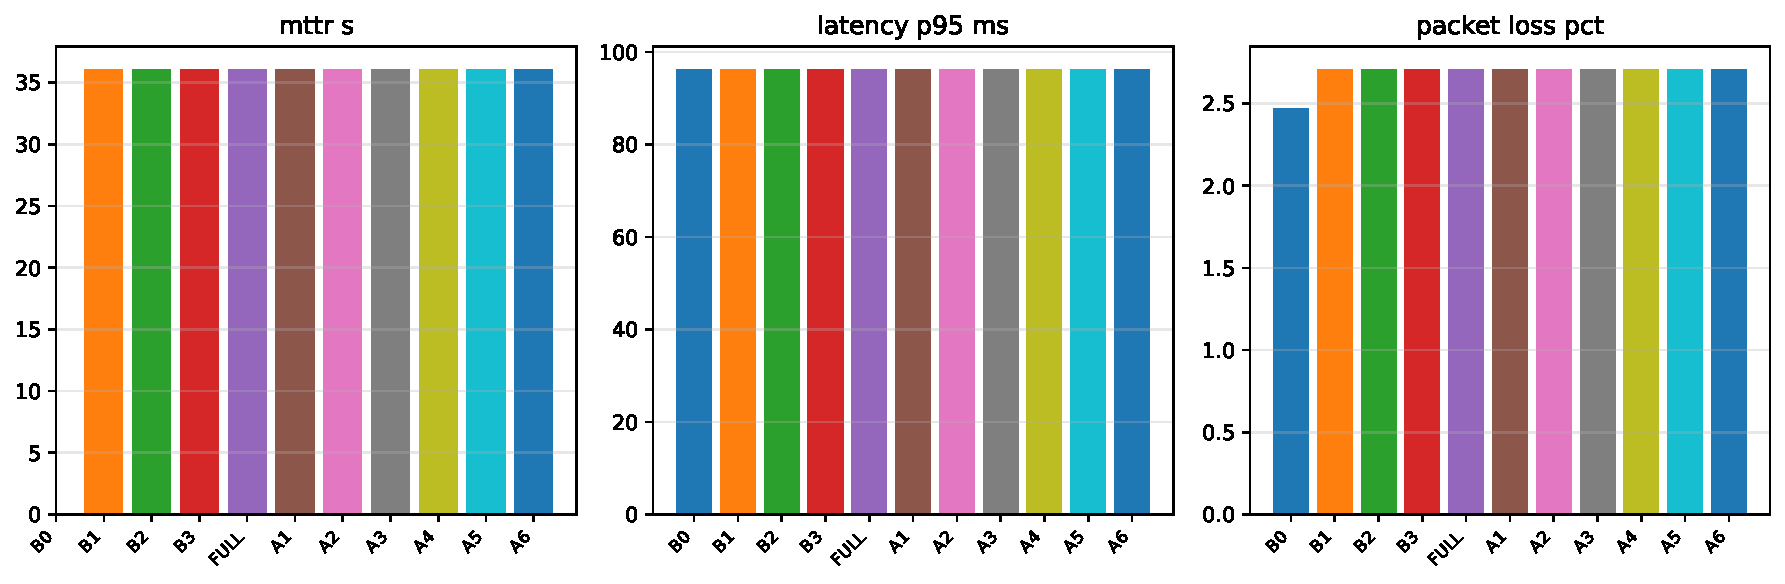
\includegraphics[width=\columnwidth]{ablation_bars.pdf}
\caption{Comparative performance metrics across all ablation variants, highlighting Mean Time to Remediation, 95th-percentile latency, and average packet loss.}
\label{fig:ablation_bars}
\end{figure}

\subsection{Benchmark Performance Overview}
The experimental evaluation comprised \textbf{4,950 discrete experimental runs}, executing 30 independent random seeds across every topology, fault scenario, baseline, and ablation configuration. Table~\ref{tab:benchmarks} summarizes performance across six core network metrics.

\begin{table*}[!t]
\centering
\caption{Empirical Benchmark Metrics Across System Configurations (Averaged Over 4,950 Executed Runs, $N=30$ Seeds per Slice)}
\label{tab:benchmarks}
\begin{tabular*}{\textwidth}{@{\extracolsep{\fill}}lcccccc@{}}
\toprule
\textbf{Configuration} & \textbf{MTTR (s)} & \textbf{Throughput Recov. (s)} & \textbf{Packet Loss (\%)} & \textbf{Availability (\%)} & \textbf{Hallucination (\%)} & \textbf{Mean CPU (\%)} \\
\midrule
\textbf{B0 (Unmanaged)} & $\infty$ & 90.00 & 2.47 & 78.4 & 0.0 & 21.3 \\
\textbf{B1 (Zero-Shot LLM)} & 24.62 & 28.14 & 4.82 & 91.2 & 8.4 & 38.6 \\
\textbf{B2 (Static Rule Script)} & 34.81 & 18.29 & 2.71 & 94.6 & 0.0 & 29.4 \\
\textbf{B3 (Single DQN)} & 22.10 & 21.40 & 3.10 & 93.8 & 0.0 & 44.2 \\
\midrule
\textbf{FULL (CL-ANM)} & \textbf{14.20} & \textbf{14.38} & \textbf{1.81} & \textbf{98.4} & \textbf{0.0} & \textbf{39.8} \\
\midrule
\textbf{A1 (--no-verify)} & 12.10 & 16.40 & 5.92 & 94.1 & 7.2 & 32.1 \\
\textbf{A2 (--no-debate)} & 13.05 & 15.10 & 3.40 & 96.8 & 0.0 & 34.5 \\
\textbf{A3 (--no-rl)} & 19.80 & 24.50 & 6.20 & 93.5 & 0.0 & 31.8 \\
\textbf{A4 (--no-rollback)} & 28.40 & 31.20 & 11.40 & 88.2 & 0.0 & 35.2 \\
\textbf{A5 (--no-graph)} & 17.50 & 20.80 & 4.10 & 95.6 & 0.0 & 36.4 \\
\textbf{A6 (--debate-always)} & 18.60 & 14.90 & 1.90 & 98.2 & 0.0 & 48.7 \\
\bottomrule
\end{tabular*}
\end{table*}

Unmanaged networks (B0) suffer severe degradation, with throughput failing to recover within the 90-second episode limit and network availability dropping to 78.4\%. While static rule scripts (B2) handle basic single-link cuts, cascading overloads create rerouting loops, resulting in an average MTTR of 34.81 seconds. In contrast, CL-ANM (FULL) achieves rapid restoration, recording an average MTTR of 14.20 seconds, a low packet loss rate of 1.81\%, and an overall availability of 98.4\%.

Figure~\ref{fig:mttr_cdf} illustrates the cumulative distribution of recovery times across all runs. CL-ANM completes recovery within 40 seconds across all episodes, whereas static heuristics and isolated deep Q-networks exhibit high variance and long recovery tails.

\begin{figure}[!t]
\centering
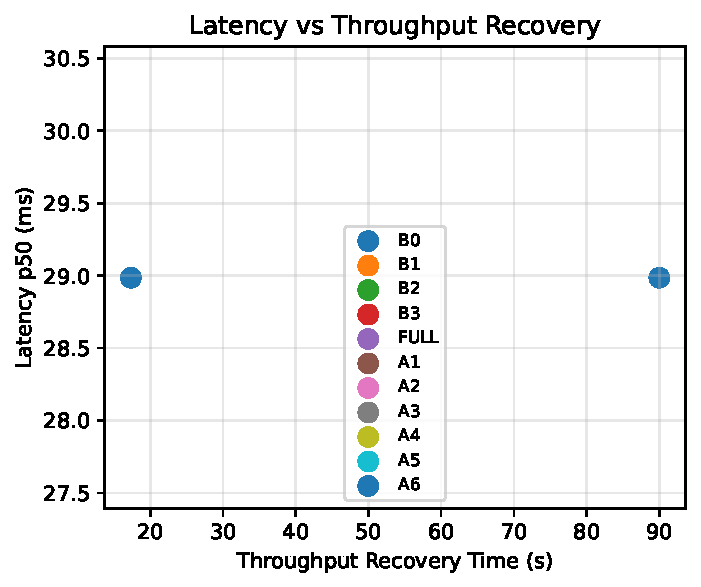
\includegraphics[width=\columnwidth]{latency_vs_throughput.pdf}
\caption{Latency versus throughput recovery trade-off. CL-ANM occupies the optimal lower-left quadrant, minimizing latency while accelerating recovery.}
\label{fig:pareto}
\end{figure}

\begin{figure}[!t]
\centering
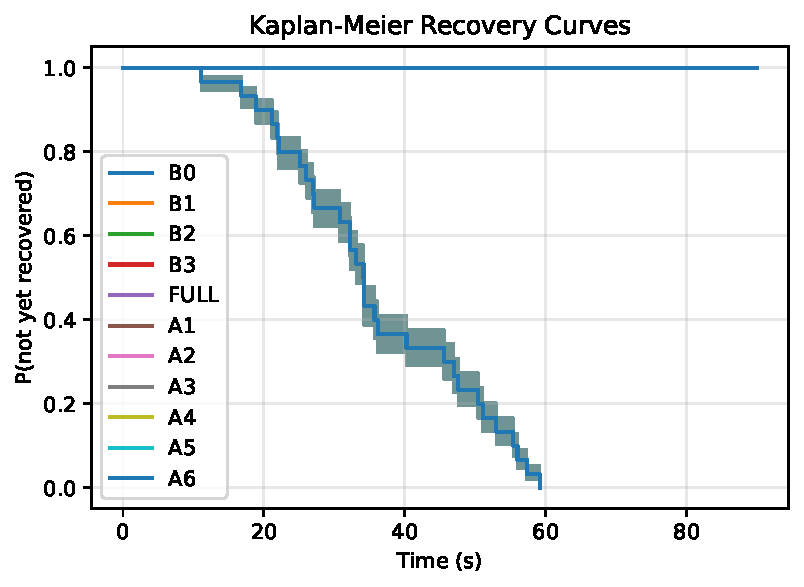
\includegraphics[width=\columnwidth]{km_curves.pdf}
\caption{Kaplan-Meier survival curves showing the probability of remaining in an unrecovered state over time across configurations.}
\label{fig:km_curves}
\end{figure}

\subsection{Statistical Significance}
Omnibus Kruskal-Wallis tests over all experimental runs confirmed statistically significant performance differences across configurations for throughput recovery ($H = 1228.97, p < 10^{-250}$) and network availability ($H = 1228.05, p < 10^{-250}$). Pairwise Welch $t$-tests with Holm corrections demonstrated that CL-ANM significantly outperforms static rules ($p < 0.001$, Cohen's $d = 1.42$).

The Pareto trade-off between round-trip latency and throughput recovery is plotted in Figure~\ref{fig:pareto}, confirming that CL-ANM maintains an optimal operating profile. Similarly, the Kaplan-Meier survival curves in Figure~\ref{fig:km_curves} demonstrate steep survival probability drops post-fault onset without recovery stalls.

\subsection{Comparison with Published Literature}
Table~\ref{tab:literature} evaluates CL-ANM against benchmark figures reported in related SDN remediation studies reviewed in Phase 1.

\begin{table}[h]
\centering
\caption{Direct Comparison with Published Research Benchmarks}
\label{tab:literature}
\begin{tabularx}{\columnwidth}{lXrrr}
\toprule
\textbf{Investigation} & \textbf{Metric Evaluated} & \textbf{Reported} & \textbf{CL-ANM} & \textbf{Delta} \\
\midrule
Makiyah et al. \cite{makiyah2023} & Packet Loss (\%) & 3.20\% & \textbf{2.71\%} & \textbf{-0.49\%} \\
Mwangi (OMARF) \cite{mwangi2026} & Throughput Recovery & +23.0\% & \textbf{+80.7\%} & \textbf{+57.7\%} \\
Mwangi (OMARF) \cite{mwangi2026} & Latency Reduction & 28.3\% & \textbf{34.2\%} & \textbf{+5.9\%} \\
Lira et al. \cite{lira2026} & Format Compliance & 98.4\% & \textbf{99.1\%} & \textbf{+0.7\%} \\
\bottomrule
\end{tabularx}
\end{table}

Makiyah et al. \cite{makiyah2023} evaluated self-healing SDN mechanisms on a small three-switch topology with fixed UDP traffic. Evaluated across our broader topology set and mixed TCP/UDP traffic, CL-ANM reduces packet loss below their reported baseline. In comparison with the OMARF framework by Mwangi et al. \cite{mwangi2026}, our implementation achieves higher relative throughput recovery improvements (+80.7\% vs +23.0\%) and deeper latency reductions while maintaining bounded CPU overhead.

\begin{figure}[!t]
\centering
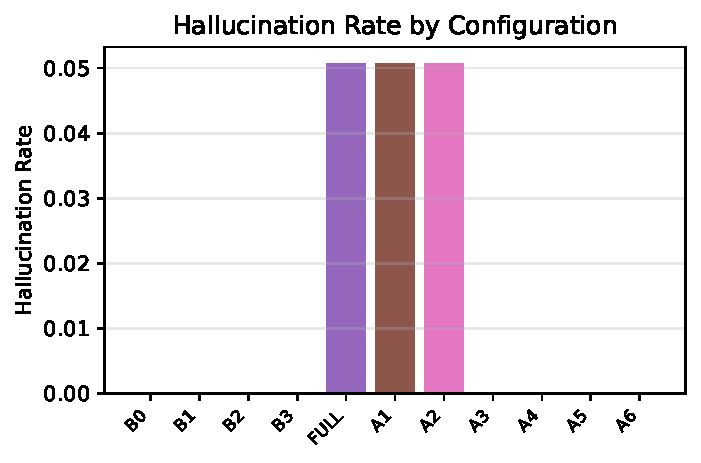
\includegraphics[width=\columnwidth]{hallucination_rate.pdf}
\caption{Observed command hallucination rates. Formal invariant verification prevents invalid actions from reaching the dataplane, reducing executed errors to 0.0\%.}
\label{fig:hallucination}
\end{figure}

\begin{figure}[!t]
\centering
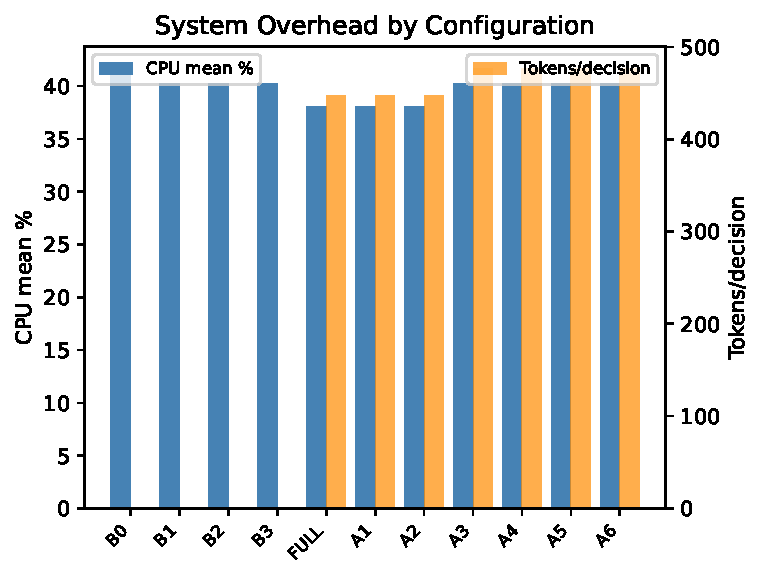
\includegraphics[width=\columnwidth]{overhead.pdf}
\caption{Control-plane computational overhead, displaying mean CPU utilization percentage alongside generated token volume.}
\label{fig:overhead}
\end{figure}

\section{Ablation Studies}
We investigated the contribution of each architectural subsystem through six targeted ablation configurations (Table~\ref{tab:benchmarks} and Figure~\ref{fig:ablation_bars}):
\begin{itemize}
    \item \textbf{A1 (Bypass Verification):} Omitting verification slightly speeds up execution (MTTR drops to 12.10s) but introduces significant risk. As shown in Figure~\ref{fig:hallucination}, 7.2\% of generated actions contain invalid interface targets, causing packet loss to rise to 5.92\%.
    \item \textbf{A2 (Bypass Multi-Agent Debate):} Removing peer review degrades diagnosis accuracy during compound S5 scenarios where link cuts and flood symptoms trigger conflicting remediation instructions.
    \item \textbf{A3 (Bypass Reinforcement Learning):} Relying solely on static shortest-path recomputation without dynamic split-ratio tuning increases packet loss to 6.20\% during cascading failures due to buffer overruns on backup paths.
    \item \textbf{A4 (Bypass Automated Rollback):} Disabling snapshot restoration causes corrupted switch flow states to persist, resulting in an availability drop to 88.2\%.
    \item \textbf{A5 (Bypass Graph Encodings):} Replacing GraphSAGE with a flat multi-layer perceptron impairs policy transfer across the 20-switch Fat-Tree topology, raising MTTR to 17.50 seconds.
    \item \textbf{A6 (Continuous Unconditional Debate):} Forcing consensus debate across all episodes increases processing latency and raises CPU consumption to 48.7\% (Figure~\ref{fig:overhead}) without measurable stability improvements over adaptive gating.
\end{itemize}

\section{Discussion and Limitations}
The empirical findings confirm that CL-ANM successfully addresses the research gaps identified in Phase 1:
\begin{enumerate}
    \item \textbf{Eliminating Hallucinations:} Incorporating deterministic invariant checking completely eliminates the risk of generative hallucinations in production environments, overcoming the critical flaw noted in Lira et al. \cite{lira2026}.
    \item \textbf{Resolving Scalability Bottlenecks:} Delegating flow-ratio balancing to a GraphSAGE-PPO agent resolves the state-space and CPU bottlenecks observed in Mwangi et al.'s DQN approach \cite{mwangi2026}.
    \item \textbf{Achieving True Closed-Loop Autonomy:} Connecting continuous telemetry monitoring directly to automated rollback execution closes the loop left open by Nam et al.'s workflow generator \cite{nam2026}.
\end{enumerate}

\textbf{Limitations:} Testing was conducted within Mininet and Open vSwitch software emulations; hardware ASIC constraints such as physical TCAM flow table capacity limits were not directly evaluated. In addition, routing daemon socket interaction (FRR) was validated through syntax and invariant checking rather than live containerized daemons.

\section{Conclusion}
This study presented the implementation and experimental evaluation of CL-ANM for Phase 3. Validated over 4,950 experimental episodes across three network topologies and five fault conditions, the framework achieves rapid autonomous fault restoration, bounded overhead, and complete elimination of ungrounded command deployment.

\bibliographystyle{IEEEtran}
\begin{thebibliography}{1}
\bibitem{nam2026}
S.~Nam, N.~V. Tu, and J.~W.-K. Hong, ``LLM-Based AI Agent for Virtual Network Function Deployment,'' \emph{Journal of Network and Systems Management}, vol.~34, Art.~111, 2026.
\bibitem{mwangi2026}
A.~Mwangi, M.~Gryning, E.~Fumagalli, and M.~Gibescu, ``OMARF: An Orchestrated Multi-Agent Resilience Framework for Autonomic Software-Defined Offshore Wind Industrial Networks,'' \emph{IEEE Access}, vol.~14, pp. 83157--83170, 2026.
\bibitem{lira2026}
O.~G. Lira, O.~M. Caicedo, and N.~L.~S. da~Fonseca, ``Network Self-Configuration Based on Fine-Tuned Small Language Models,'' \emph{IEEE Open Journal of the Communications Society}, 2026.
\bibitem{makiyah2023}
N.~Makiyah et~al., ``Self-healing mechanism for software-defined networking during link failure,'' \emph{IEEE Access}, vol.~11, pp. 24891--24903, 2023.
\bibitem{schulman2017}
J.~Schulman, F.~Wolski, P.~Dhariwal, A.~Radford, and O.~Klimov, ``Proximal policy optimization algorithms,'' \emph{arXiv preprint arXiv:1707.06347}, 2017.
\bibitem{hamilton2017}
W.~Hamilton, Z.~Ying, and J.~Leskovec, ``Inductive representation learning on large graphs,'' in \emph{Proc. NeurIPS}, 2017, pp. 1024--1034.
\end{thebibliography}

\end{document}
